\documentclass[12pt,a4paper]{article}
\usepackage[utf8]{inputenc}
\usepackage[spanish]{babel}
\usepackage{amsmath}
\usepackage{amsfonts}
\usepackage{amssymb}
\usepackage{latexsym}
\usepackage{makeidx}
\usepackage{graphicx}
\usepackage{graphics}
\usepackage{lmodern}
\usepackage{hyperref}
\usepackage{subcaption}
\usepackage{pgfplots}
\usepackage{dsfont}
\usepackage{multicol}
\usepackage{xcolor}
\usepackage{booktabs}
\usepackage{float}
\usepackage{subcaption}
\pgfplotsset{width=10cm,compat=1.9}
\usepgfplotslibrary{external}
\usepackage{fancybox}
\usepackage{subcaption}
\usepackage{xcolor, colortbl}


\setlength{\parindent}{0px}
\usepackage[left=2cm,right=2cm,top=4cm,bottom=2cm]{geometry}

\author{Daniel Vázquez Lago}
\title{Estudio de un circuito RLC en serie}

\newcommand{\parentesis}[1]{\left( #1  \right)}
\newcommand{\parciales}[2]{\frac{\partial #1}{\partial #2}}
\newcommand{\pparciales}[2]{\parentesis{\parciales{#1}{#2}}}
\newcommand{\ccorchetes}[1]{\left[ #1  \right]}
\newcommand{\D}{\mathrm{d}}
\newcommand{\sech}{\mathrm{sech} \ }
\newcommand{\csch}{\mathrm{csch} \ }
\newcommand{\Real}{\mathrm{Re} }
\newcommand{\KHz}{\mathrm{kHz} }
\newcommand{\Hz}{\mathrm{Hz} }
\newcommand{\tquad}{\quad \quad \quad}

\definecolor{color2}{rgb}{1, 1, 1}
%\definecolor{color2}{rgb}{0.88, 0.97, 0.75}
\definecolor{color1}{rgb}{0.93, 0.93, 0.93}

\definecolor{color4}{rgb}{1, 1, 1}
%\definecolor{color4}{rgb}{0.68, 0.84, 0.99}
\definecolor{color3}{rgb}{0.93, 0.93, 0.93}

\begin{document}

\maketitle
\newpage

\tableofcontents

\newpage

\section{Objetivos}

En esta práctica trataremos de obtener experimentalmente la curva de impedancia de un circuito RLC en función de la frecuencia, calculando así el módulo y argumento de la impedancia. Además obtendremos el factor de Calidad de nuestro circuito y los parámetros  característicos de nuestro circuito (R,L,C,B...). El fin será comparar los resultados con el valor teórico para comprobar así si la teoría de circuitos que estudiamos es una buena aproximación o no de los resultados experimentales. 

\section{Introducción}

En un circuito de corriente alterna existen ciertos elementos que modifican el comportamiento de la corriente. Estos elementos son: Resistencia (R), Autoinducción (L) y condensador (C), y el circuito más básico que los contenga se llama circuito RLC (los conecta en serie entre sí). El paso de una corriente alterna por estos genera una respuesta de los mismos que afecta al propio circuito, por ejemplo disipando potencia (resistencia), generando un desfase entre voltaje e intensidad (autoinducción y condensador). Suponiendo un circuito completamente ideal, las respuestas que generan estos elementos son:

\begin{itemize}
\item \textbf{Resistencia:} disipa potencia y no cambia la fase entre $I$ y $V$. La potencia entre sus bornes vendrá dada por:

\begin{equation}
V_R(t) = \Real [R I_0 e^{jwt}]
\end{equation}

\item \textbf{Autoiducción:} no disipa potencia pero genera un cambio de fase entre $I$ y $V$ tal que $I$ está atrasada $\pi/2$ la fase respecto $V$ (o el voltaje está adelantado). Eso significa que:

\begin{equation}
V_L (t) = \Real [L j w I_0 e^{jwt}] 
\end{equation}


\item \textbf{Condensador:} no disipa la potencia pero genera un cambio de fase entre           $I$ y $V$ de tal forma que $I$ está adelantada una fase de $\pi/2$ respecto $V$ (o $V$ está atrasada). Viene dada por:

\begin{equation}
V_C (t) = \Real \ccorchetes{ \dfrac{1}{jwC} I_0 e^{jwt} }
\end{equation}

\end{itemize}


Entonces podemos aplicar la ley de Kirchoff de mallas para un circuito en serie, ya que la longitud del circuito es muy pequeña y las frecuencias que usamos también (del orden de $kHz$), por lo que:

\begin{equation}
V(t)  = V_R + V_L + V_C = \Real \ccorchetes{R I_0 e^{jwt} + L j w I_0 e^{jwt} +\dfrac{1}{jwC} I_0 e^{jwt} } 
\end{equation} 

donde podemos agrupar los términos cosenos y senos en un solo ``oscilador'', de tal forma que: 

\begin{equation}
V(t) = |Z| I_0 cos(wt+ \phi) \label{Ec:leyOhmCA}
\end{equation}

que es una relación similar a la ley de Ohm, pero para circuitos de corriente alterna. Antes de continuar voy a permitirme una breve aclaración: esto lo hemos hecho suponiendo que $I(t)=I_0 cos(wt)$. Sin embargo realmente es el potencial el que se comporta como $V(t)=V_0 cos(wt)$ (ya que está dada por un generador, luego es la intensidad la que cambia de fase y de módulo). Aunque a la hora de la verdad no nos importa (es hacer un cambio de variables y ya), tenemos que realmente:

\begin{equation}
I (t) = \dfrac{V}{Z} = \dfrac{V_0}{|Z|} cos(wt - \phi)
\end{equation} \\

Acabada esta aclaración, definimos la \textbf{impedancia} del circuito como el número complejo:

\begin{equation}
Z(w) = R + j \parentesis{ wL - \dfrac{1}{wC}}
\end{equation}

De tal modo que en la ecuación \ref{Ec:leyOhmCA} tenemos que:

\begin{equation}
|Z(w)| = \sqrt{R^2 + \parentesis{wL- \frac{1}{wC}}^2}  \tquad \phi = \arg(Z) = \arctan \parentesis{\dfrac{wL-(1/wC)}{R}} \label{Ec:z-y-arg(z)}
\end{equation}

Llamamos al factor que va con el número complejo (responsable del desfase)  \textbf{reactancia}. Una vez hemos llegado hasta aquí podemos entender el significado físico de la impedancia: es una medida del desfase entre intensidad y voltaje en un circuito RLC, además de darnos una medida de como se relacionan las amplitudes de ambos. En general es una medida de la oposición del circuito a la corriente alterna.  Ahora podemos definir los siguientes parámetros:

\begin{itemize}
\item \textbf{Frecuencia de resonancia:} llamamos frecuencia de resonancia a la frecuencia $w$ tal que no hay desfase. Teoricamente vendrá dado por:

\begin{equation}
w_0 = \dfrac{1}{\sqrt{LC}}
\end{equation}

\item \textbf{Factor de Calidad:} el factor de calidad se define como el cociente entre la energía que se puede almacenar en un circuito RLC y la disipada, por un factor $2 \pi$. En un circuito RLC viene dado por:

\begin{equation}
Q =  \dfrac{w_0 L}{R}
\end{equation}

\item \textbf{Banda de paso:} se le llama así a la longitud del intervalo donde la curva de amplitud cae un $1/\sqrt{2}$ respecto su valor máximo. Viene dado por:

\begin{equation}
B = \dfrac{w_0}{2 \pi Q}
\end{equation}
\end{itemize}


Como podemos ver existe un gran paralelismo entre lo estudiando con un oscilador armónico forzado y un circuito RLC. Esto es porque la ecuación del circuito viene dada por:

\begin{equation}
V_0  \cos(w t) =  L \dfrac{\D I}{\D t} + \dfrac{Q}{C} + IR  \Longrightarrow  L \ddot{Q} + R \dot{Q} + C^{-1} Q = V_0 \cos (wt)
\end{equation}

\section{Material}


Nuestro material será:

\begin{itemize}
\item \textbf{Placa RLC:} contendrá una pequeña bobina (autoinductancia $L$), un condensador (capacidad $C$) y una resistencia $R_T$ que vendrá dada por la suma de la resistencia de la bobina y una resistencia externa. Aunque en la propia placa de RLC no nos vengan dadas las incertidumbres del material, tenemos que el guión nos dice que una tolerancia adecuada para estos valores es una entorno al $3 \thicksim 5\%$. Por lo tanto tomaremos una tolerancia del $ 5 \%$ para la autoinductancia de la bobina, y una del $3\%$ para la capacidad del condensador. Las incertidumbres de las resistencias se tomarán con el polímetro. Ver figura \ref{Fig:placa-RLC} \footnote{Autoría de la foto: Sara Gonzalez, Práctica 2018.}. 

\item \textbf{Generador de corriente alterna:} nuestro generador de corriente, que aportará un potencial tal que $V(t) = V_0cos(wt)$.


\item \textbf{Osciloscopio:} nuestro osciloscopio será un ``Osciloscopio Siglent SDS 1102CML''. No incluimos todas las incertidumbres que nos da la hoja de especificaciones (ya que las medidas dependen de la escala y otros factores que no conocemos), una incertidumbre razonable será la incertidumbre combinada del $5\%$ de la medida mas un factor $0.1 V$ o $2 mV$. Está última solo la usaremos si el voltaje es inferior a $1V$, ya que es lo que nos indica el fabricante. 


\item \textbf{Polímetro:} nuestro polímetro no tiene especificaciones exactas. De todos modos aunque no conozcamos la incertidumbre exacta de nuestro fabricante, vamos a usar la incertidumbre que ya conocemos para la mayoría de los polímetros del laboratorio de electromagnetismo. En general una buena aproximación de la incertidumbre será de:

$$ s(R) \equiv 0.5 \%  + 2$$


\begin{figure}[h!] \centering
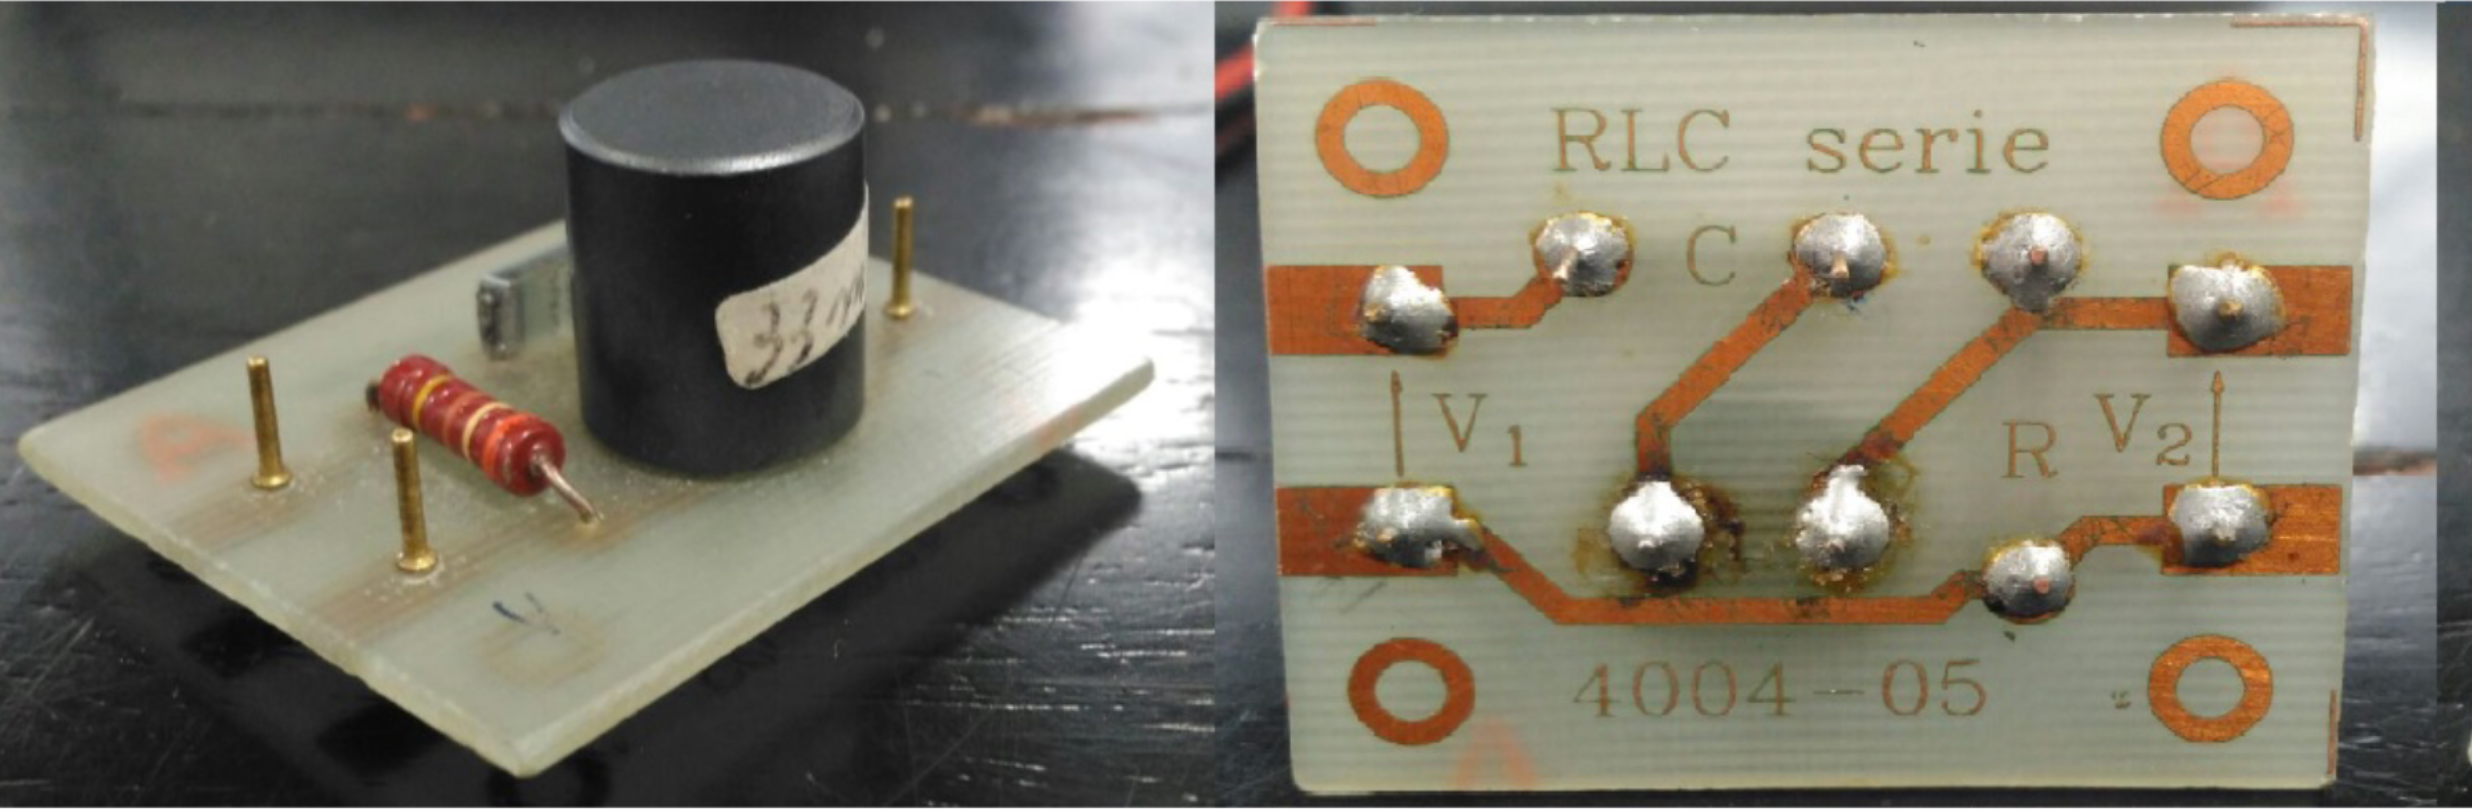
\includegraphics[scale=0.4]{RLC.png}
\caption{Imagen de nuestra placa RLC}
\label{Fig:placa-RLC}
\end{figure}


\end{itemize}

\newpage

\section{Procedimiento experimental}

Lo primero que haremos nada mas llegar al laboratorio será medir la resistencia de nuestro circuito con un polímetro, para luego calcular algunos valores teóricos como $w_0$ para poder orientarnos mejor al comenzar a tomar datos. \\

Una vez tenemos esto lo que haremos será conectar el osciloscopio al generador directamente y luego al circuito RLC, de tal forma que le lleguen dos señales diferentes: una del propio generador ($V_1$), sin desfasar, y otra tras desfasarse por culpa del circuito RLC ($V_2$). Seleccionamos una onda sinusoidal en el generador, y lo  que haremos es buscar cual es la frecuencia de resonancia experimental, buscando el lugar donde el desfase es cero, y la potencia $V_2$ es máxima. Podemos comenzar con la teórica para luego ajustar. Todos los datos (las amplitudes de los voltajes, las frecuencias...) las medimos en el osciloscopio. En la siguiente figura se representa el esquema eléctrico. Las flechas $V_2$ y $V_1$ representan los bordes que están conectados al osciloscopio.   \\

\begin{figure}[h!] \centering
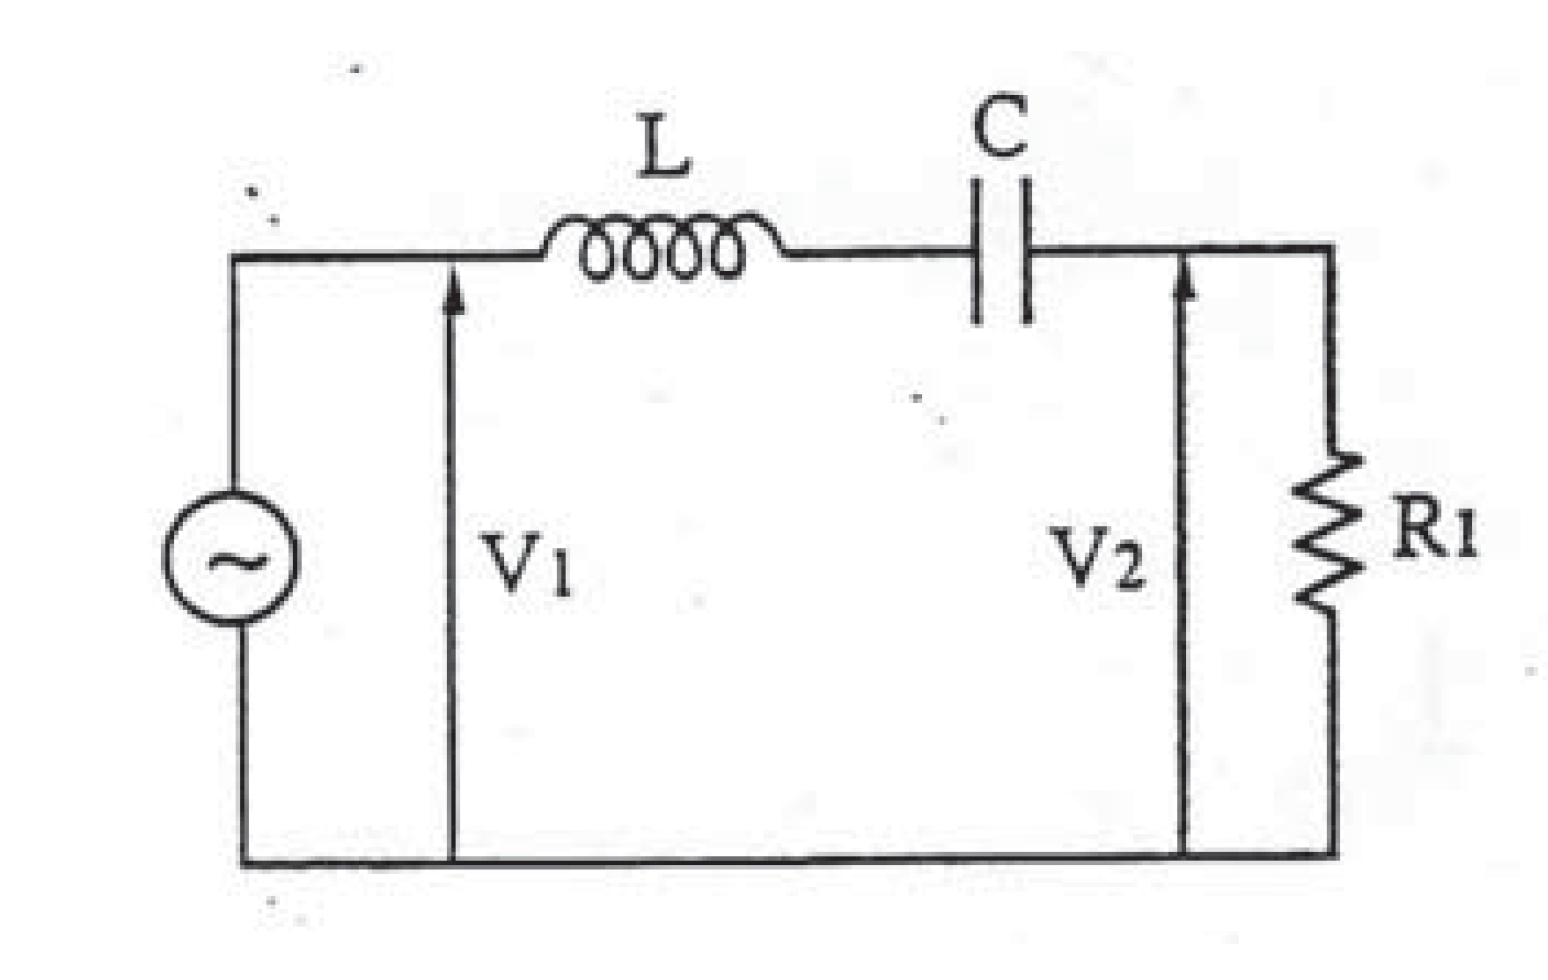
\includegraphics[scale=0.3]{RLC2.png}
\caption{esquema eléctrico. Foto presentada en el guion de la práctica.}
\end{figure}

A partir de esta frecuencia de resonancia iremos aumentando las frecuencias para para encontrar desfases en intervalos de $5^o$, hasta que lleguemos a $10$kHz, donde tomaremos valores de $20,50$ y $100 \KHz$. Luego haremos exactamente lo mismo pero bajando las frecuencias, hasta llegar al entorno de $1000\Hz$, a partir del cual tomaremos $500,200,100 \Hz$. En cada uno de estos puntos tomaremos las diferencias de potencial y los desfases para la frecuencia. \\

Es vital tomar nota de la escala de tiempos que tiene el osciloscopio en cada medida, puesto que tendrá relación con la incertidumbre del desfase, tal y como explicaremos en la sección \ref{Sec:5}.

\section{Análisis de datos} \label{Sec:5}

En primer lugar vamos a explicar un poco las fuentes de incertidumbres de cada medida que hagamos en esta práctica, luego haremos todos los cálculos explicando paso por paso como vamos obteniendo los datos que buscamos.\\


La incertidumbre de las resistencias vendrán dadas por la incertidumbre del polímetro, y los voltajes por la incertidumbre del osciloscopio. La frecuencia nos sale en el osciloscopio, con una gran precisión (hasta 5 decimales). Sin embargo en general oscila mucho este valor, por ello asignaremos una incertidumbre que contenga todas las posibles variaciones de la frecuencia. Está será:

\begin{equation}
s(f) = 0.01 \KHz
\end{equation}

Ahora estudiaremos el dato con mayor incertidumbre (o al menos el que mas fuente tiene): el desfase. El problema del desfase es que tiene varias fuentes de incertidumbre, una procedente de la variación de la lectura del osciloscopio, y otra procedente de como se calcula la incertidumbre del desfase. \\

Cuando llegamos al laboratorio y tratamos de obtener un dato de desfase para determinada frecuencia, vemos que en la pantalla los datos oscilan bastante, por lo que es imposible decidir cual es el más correcto. Para realizar la toma de datos lo que haremos será lo siguiente: veremos cual es la oscilación, anotando el valor máximo y mínimo que aparecen en la pantalla durante unos 10 segundos. Luego, tomaremos el valor medio entre estos dos (su distribución de frecuencias es gaussiana) y la incertidumbre será la mitad del rango total del intervalo. \\

Para calcular el desfase, el osciloscopio lo que hace es medir la diferencia de tiempos que hay entre una señal y otra (a), por la frecuencia, de tal modo que:

\begin{equation}
\phi = 2 \pi f a
\end{equation}

Y ahora bien, ¿Cuál es la incertidumbre asociada a cada uno de estos parámetros? La frecuencia ya la hemos mencionado, luego la incertidumbre asociada a $a$ depende intrínsecamente de la escala que hemos usado para medir el desfase, por eso es sumamente importante anotarla. Esta incertidumbre entonces vendrá dada por:

\begin{equation}
s(a) = \dfrac{N \cdot \mathrm{escala}}{1000} \tquad N = 15
\end{equation}

Entonces la incertidumbre total de cada desfase vendrá dada por la incertidumbre combinada. Es importante mencionar que todas los ajustes se han hecho ponderados, usando el módulo de Python scipy.optimize.

\subsection{Parte 1}

En este apartado cogeremos los valores teóricos de la resistencia, del condensador y la autoinductancia, y luego usando las fórmulas previas calcularemos el valor teórico del factor de calidad, la frecuencia de resonancia... Sean los datos:


\begin{equation} 
\begin{array}{lllllllll}
R_T & = & 345.8 & \ \Omega &  \ \ &  s(R_T) & =  & 3.6 & \ \Omega \\ 
C & = & 22.0 & \ nF &  \ \ &  s(C) & =  & 1.1 & \ nF \\ 
L & = & 33.0 & \ mH &  \ \ &  s(L) & =  & 1.6 & \ mH \\ 
\end{array} 
\end{equation} 

Podemos obtener los parámetros de manera teórica:

\begin{equation} 
\begin{array}{lllllllll}
w_0 & = & 371 \cdot 10^{2} & \ \mathrm{rad}/s &  \ \ &  s(w_0) & =  & 13 \cdot 10^{2} & \ \mathrm{rad}/s \\ 
f_0 & = & 590 \cdot 10 & \ \Hz &  \ \ &  s(f_0) & =  & 2 \cdot 10 & \ \Hz \\ 
B & = & 166 \cdot 10 & \ s^{-1} &  \ \ &  s(B) & =  & 11  \cdot 10 & \ s^{-1} \\ 
Q & = & 3.54  &   \ & \ &  s(Q) & =  & 0.22 & \\ 
\end{array} 
\end{equation} 
 
 
\subsection{Parte 2} 

\subsubsection{Parte 2.1. Calculo de $|Z^2|$}

En esta sección vamos a obtener los valores de los parámetros $C$, $L$ y $R$ en función de los datos obtenidos. Los datos que hemos obtenido en el procedimiento son los voltajes $V_1 \equiv = V_{in}$, $V_2 \equiv V_R$ y $\phi$, asociados a una frecuencia, por lo que tendremos que usar estos datos para obtenerlos. Como sabemos la intensidad que pasa por todo el circuito es la misma, por lo que la intensidad que circula por la resistencia y por el circuito es la misma. Entonces podemos aplicar la ley de Ohm:

$$ I = \dfrac{V_2}{R} ; \ \ I = \dfrac{V_1}{Z} \Longrightarrow Z = \dfrac{V_2}{V_1} R  $$

es decir podemos obtener la impedancia de nuestro circuito para una frecuencia dada si conocemos los voltajes y la resistencia. Como estos datos los conocemos, podemos usar un ajuste de $Z$ frente a $w$ para calcular estos valores. Sabemos que:

$$ |Z|^2 = L^2 w^2 + \left[ R^2  - \dfrac{2L}{C} \right] + \dfrac{1}{C^2 w^2} $$

Entonces podemos realizar el ajuste:

\begin{equation}
|Z|^2 = a_0 \dfrac{1}{w^2} + a_1 + a_2 w^2 \label{Ec:ajuste1}
\end{equation}

donde claramente:

\begin{equation}
a_0 = \dfrac{1}{C^2} \tquad a_1 = R^2-\dfrac{2L}{C} \tquad a_2 = L^2 \label{Ec:parametros1}
\end{equation}

por lo que podemos obtener estos tres parámetros. Para comprobar que el ajuste es bueno, luego con los datos obtenidos veremos si la función es capaz de ajustar la función $1/|Z|$ con todos los datos. Entonces al hacer el ajuste \ref{Fig:plot1} podemos obtener que: \\


\begin{table}[h!] 	 \centering 
\begin{tabular}{|c|c|c|c|c|c|} 
\hline 
$a_0 \ (F^{-2}) $  & $s(a_0) \ (F^{-2})$ & $ a_1 \ (\Omega^2)$ & $s(a_1) \ (\Omega^2)$ & $a_2 \ (H^2)  $ &  $s(a_2) \ (H^2)$ \\ \hline 
$20.89 \cdot 10^{14}$  & $0.69 \cdot 10^{14}$ & $ -29.01 \cdot 10^5$ & $-0.52 \cdot 10^5 $& $11.12 \cdot 10^{-4} $ & $0.32 \cdot 10^{-4}$ \\ 
\hline
\end{tabular} 
\caption{valores del ajuste \ref{Ec:ajuste1}} 
\label{Tab:parametros1} 
\end{table} 


Lo que usando las ecuaciones \ref{Ec:parametros1} nos lleva a deducir:\\

\begin{table}[h!] 	 \centering 
\begin{tabular}{|c|c|c|c|c|c|} 
\hline 
$C \ (nF) $  & $s(C) \ (nF)$ & $ L \ (mH)$ & $s(L) \ (mH)$ & $R_T \ (\Omega)  $ &  $s(R_T) \ (\Omega)$ \\ \hline 
$21.88 $  & $0.36 $ & $ 33.35$ & $0.48  $& $383  $ & $88 $ \\ 
\hline
\end{tabular} 
\caption{parámetros intrínsecos del circuito para el ajuste \ref{Ec:ajuste1}} 
\label{Tab:valores1} 
\end{table} 
 
 


Con estos valores podemos obtener tanto $Q$, $B$, $w_0$ y $f_0$: \\

\begin{table}[h!] 	 \centering 
\begin{tabular}{|c|c|c|c|c|c|c|c|} 
\hline 
$Q \  $  & $s(Q) \ $ & $ B \ (k \Hz)$ & $s(B) \ (k \Hz)$ & $w_0 \ (\mathrm{rad}/s)  $ &  $s(w_0) \ (\mathrm{rad}/s)$  & $f_0 \ (k$Hz) & $s(f_0) \  (k$Hz) \\ \hline 
$3.22 $  & $0.75 $ & $ 1.83 $ & $0.43$ & $37.02 \cdot 10^3  $ & $0.81 \cdot 10^3 $ & 5.89 & 0.13 \\ 
\hline
\end{tabular} 
\caption{parámetros intrínsecos del circuito para el ajuste \ref{Ec:ajuste1}} 
\label{Tab:valores2} 
\end{table} 
 
Las regresiones que se pueden ver como en las figuras \ref{Fig:plot1} y \ref{Fig:plot2} le faltan algunos datos extremos, que en la tabla de datos estarán marcados. Esto es porque con algunos datos extremales dada su altísima incertidumbre, alteran drásticamente la regresión, haciéndola incalculable. Por lo tanto nos hemos visto en la necesidad de no usar algunos datos en la regresión. Además incluimos la figura \ref{Fig:plot3} para que si se puedan ver los todos los datos sin las incertidumbres y además de usar la frecuencia. 

\begin{figure}[h!] \centering 
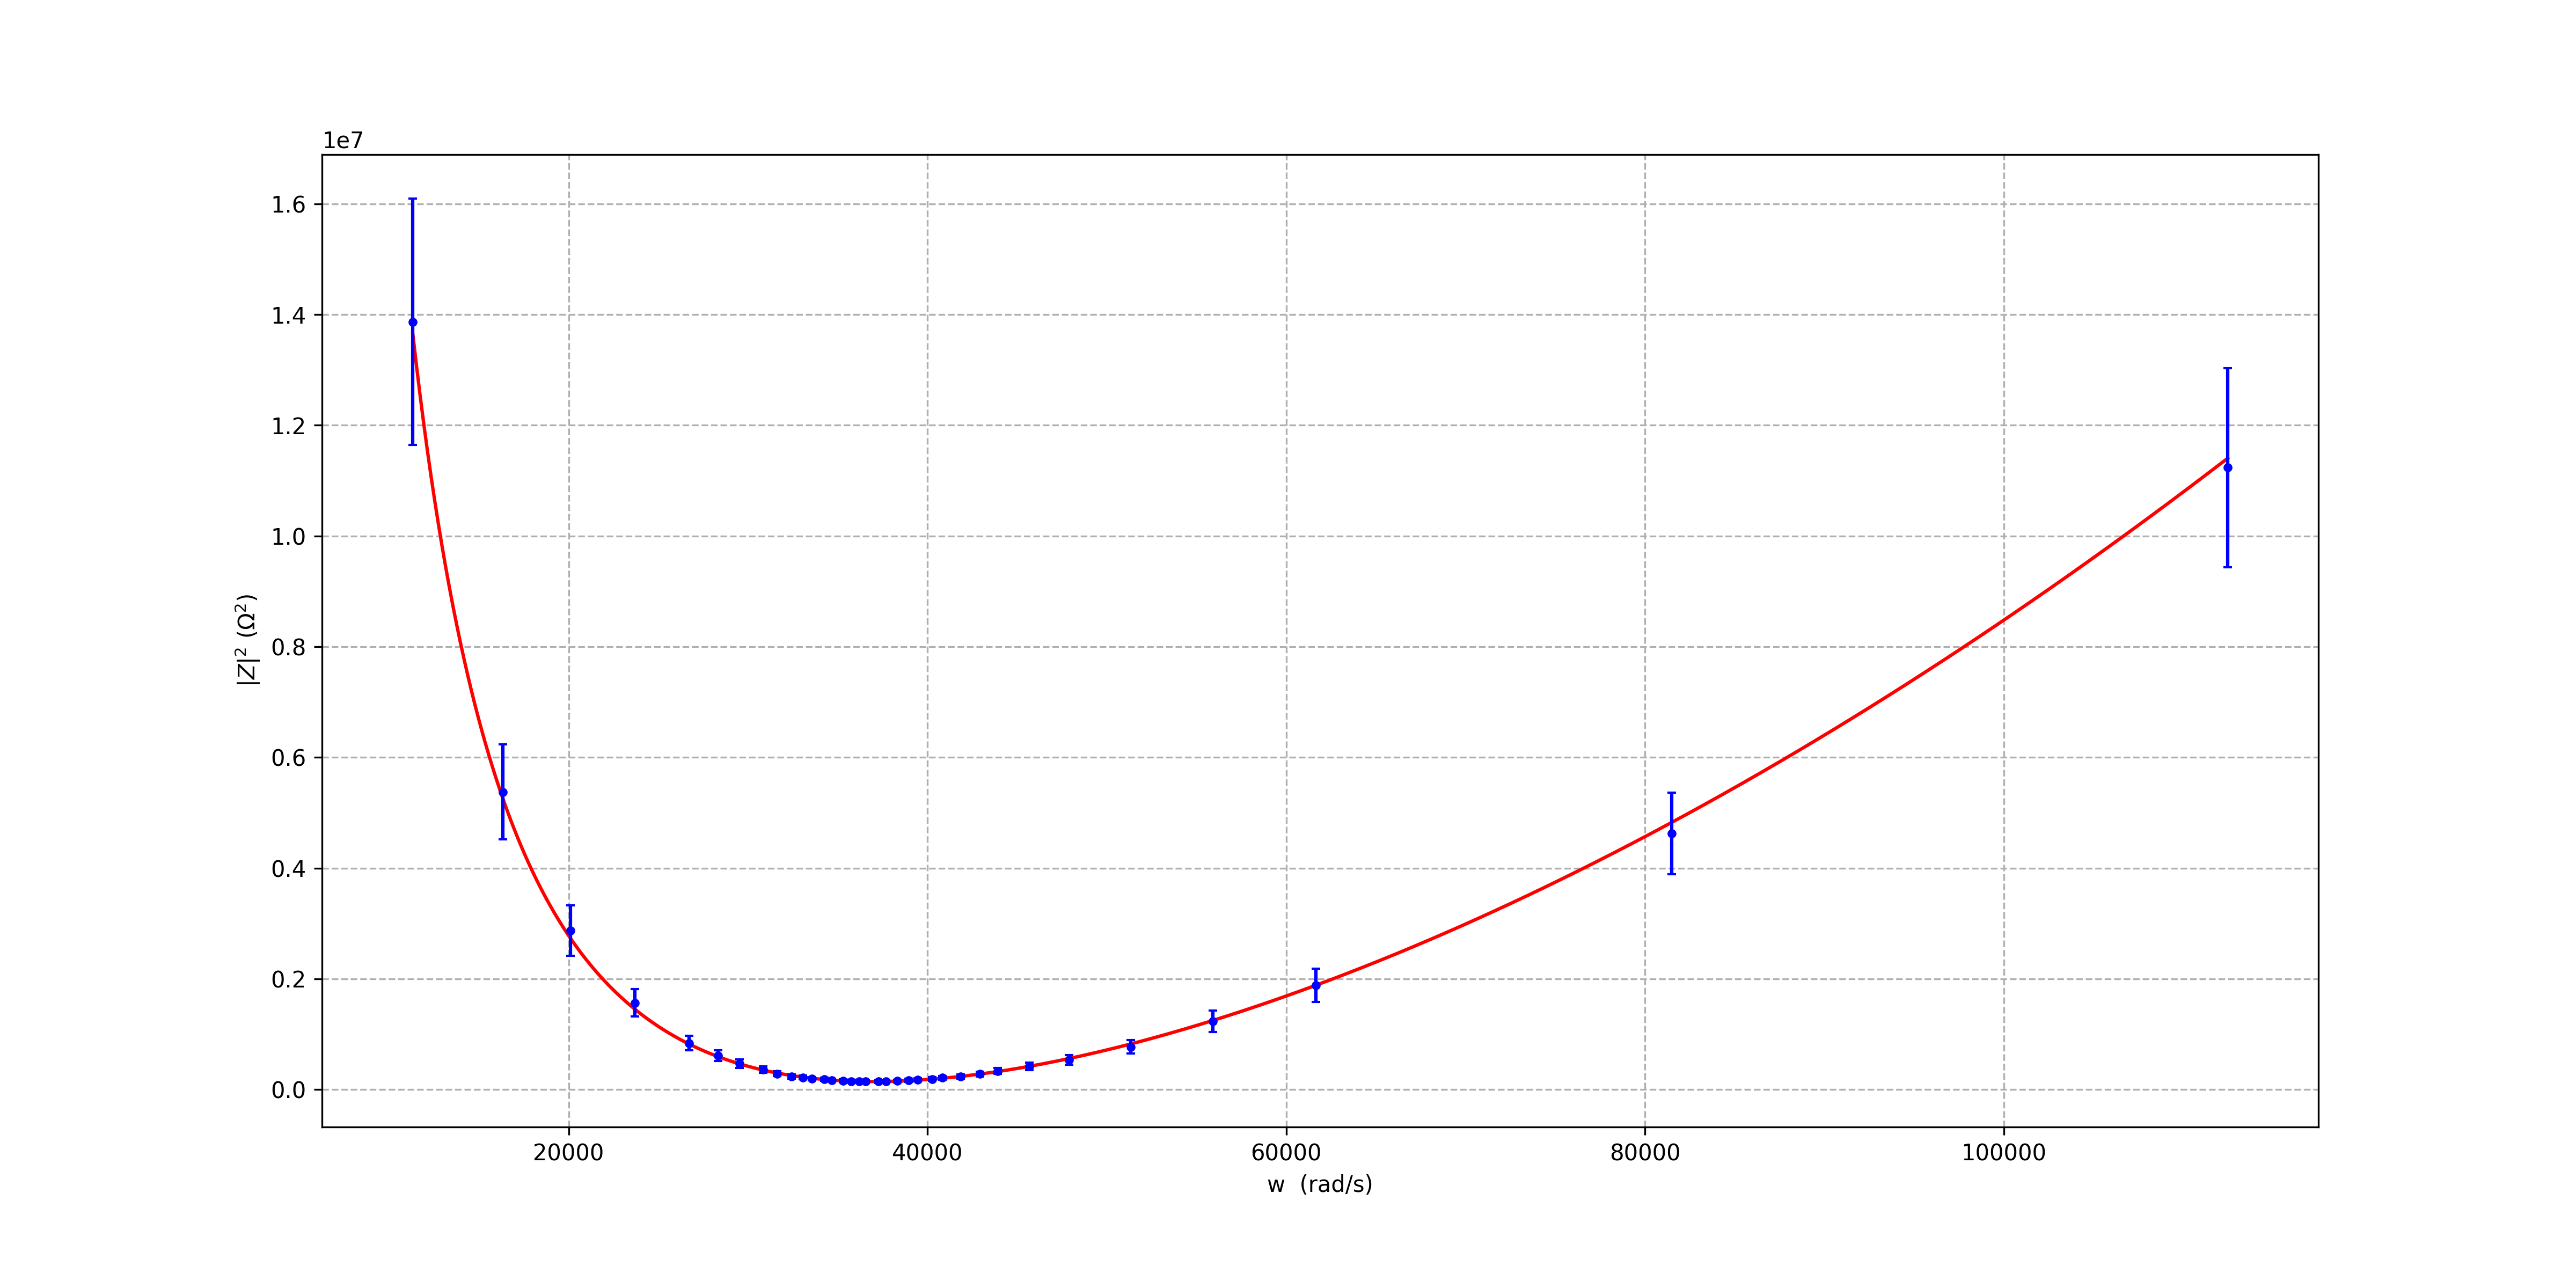
\includegraphics[scale=0.45]{plot1.png}
\caption{Ajuste a la ecuación \ref{Ec:ajuste1} de $|Z|^2$ frente a $w$.}
\label{Fig:plot1}
\end{figure}
 
\begin{figure}[h!] \centering
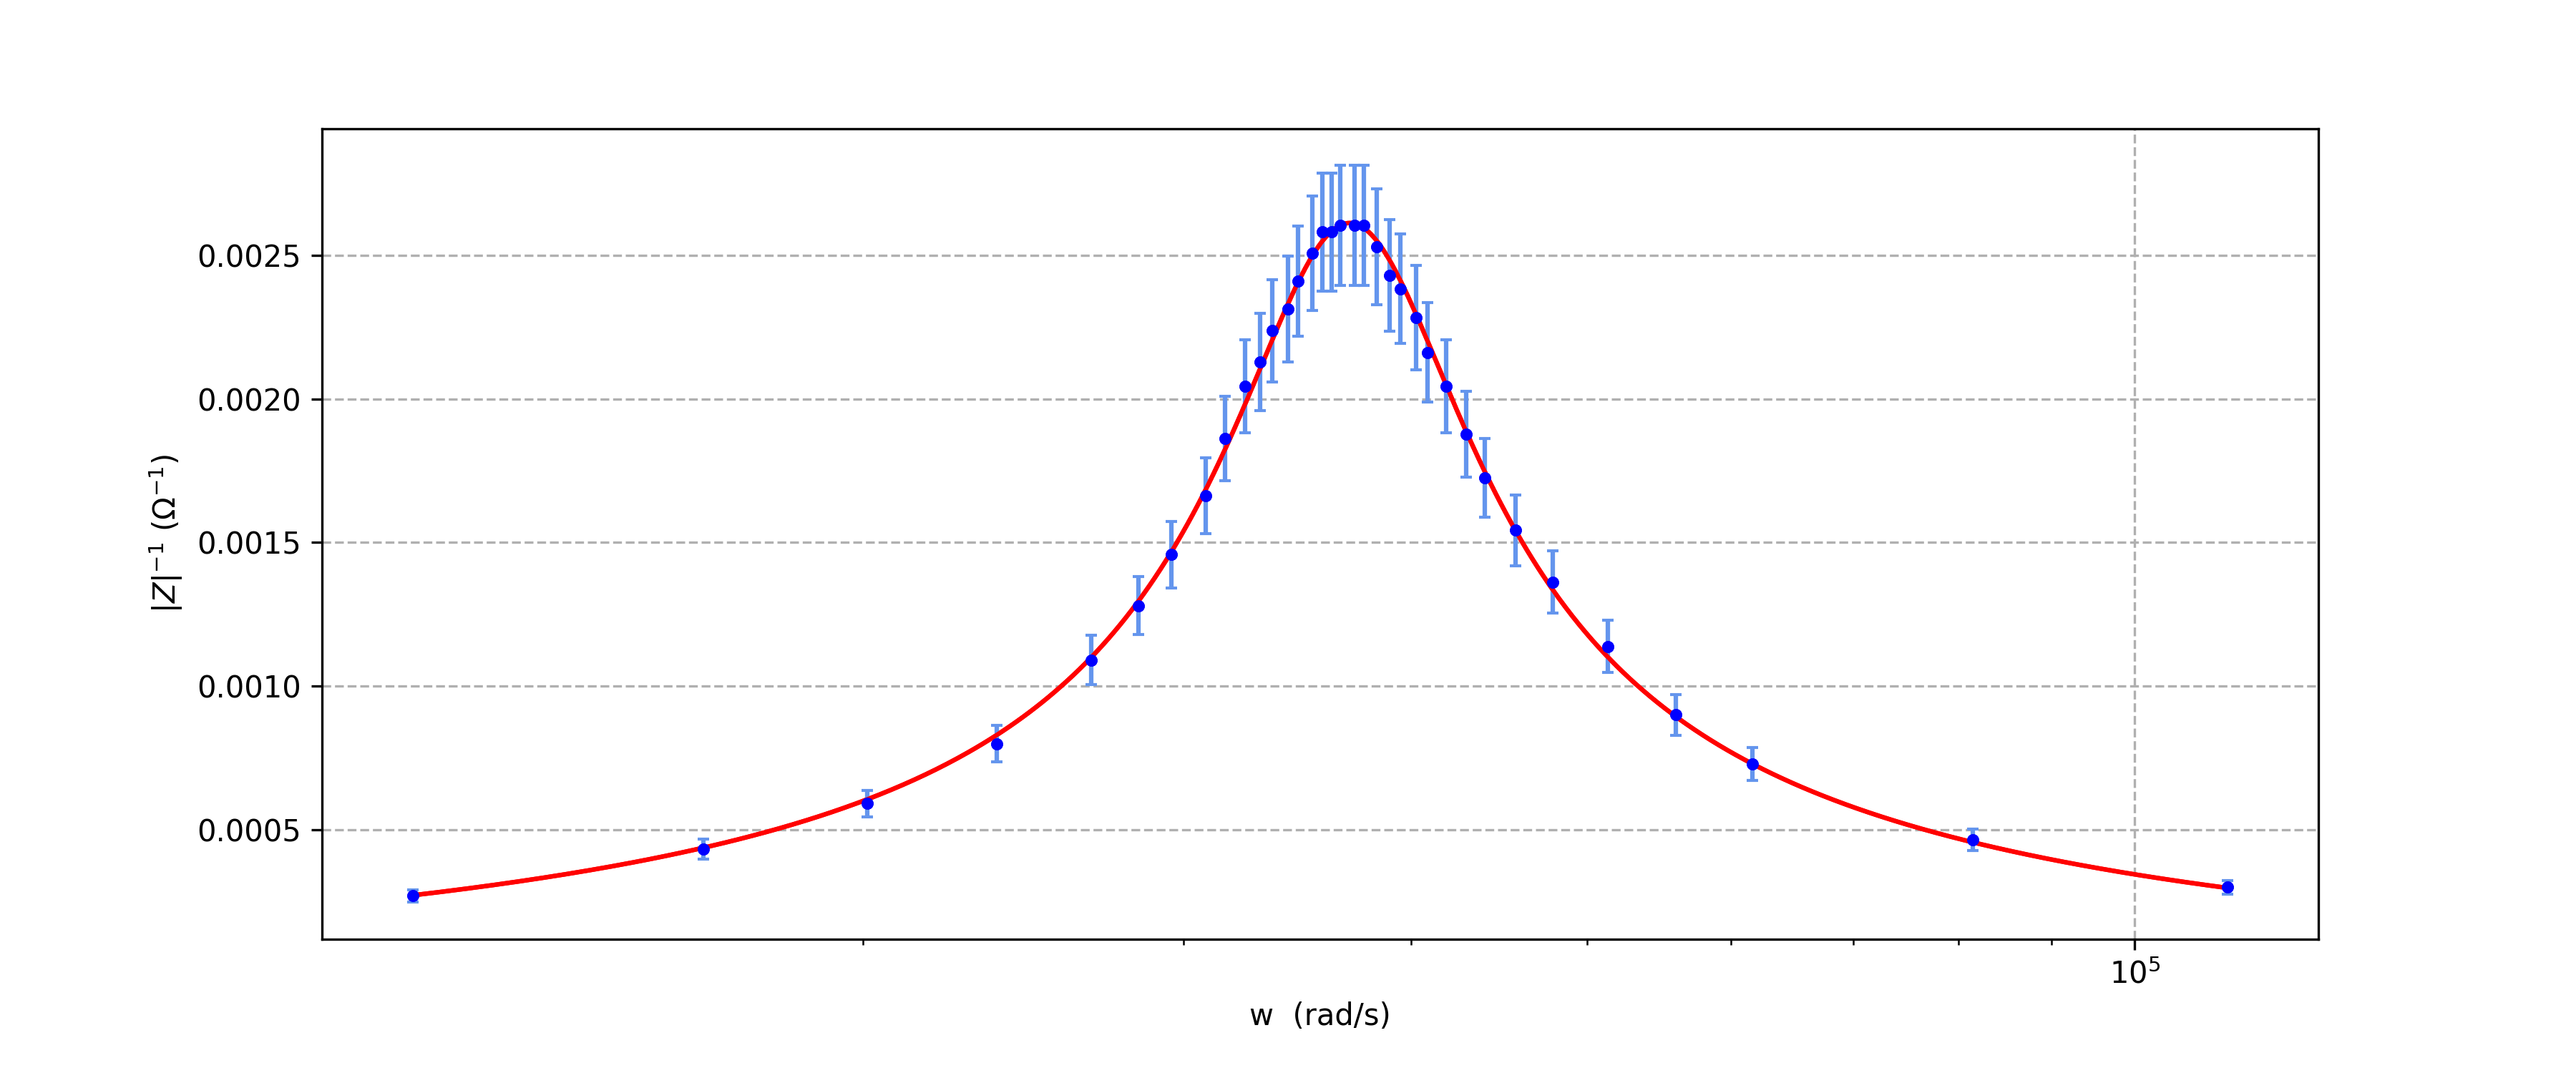
\includegraphics[scale=0.60]{plot2.png}
\caption{Representación de $|Z|^{-1}$ frente a $w$, con barras de error y escala semi-logarítmica.}
\label{Fig:plot2}
\end{figure}
 
\begin{figure}[h!] \centering
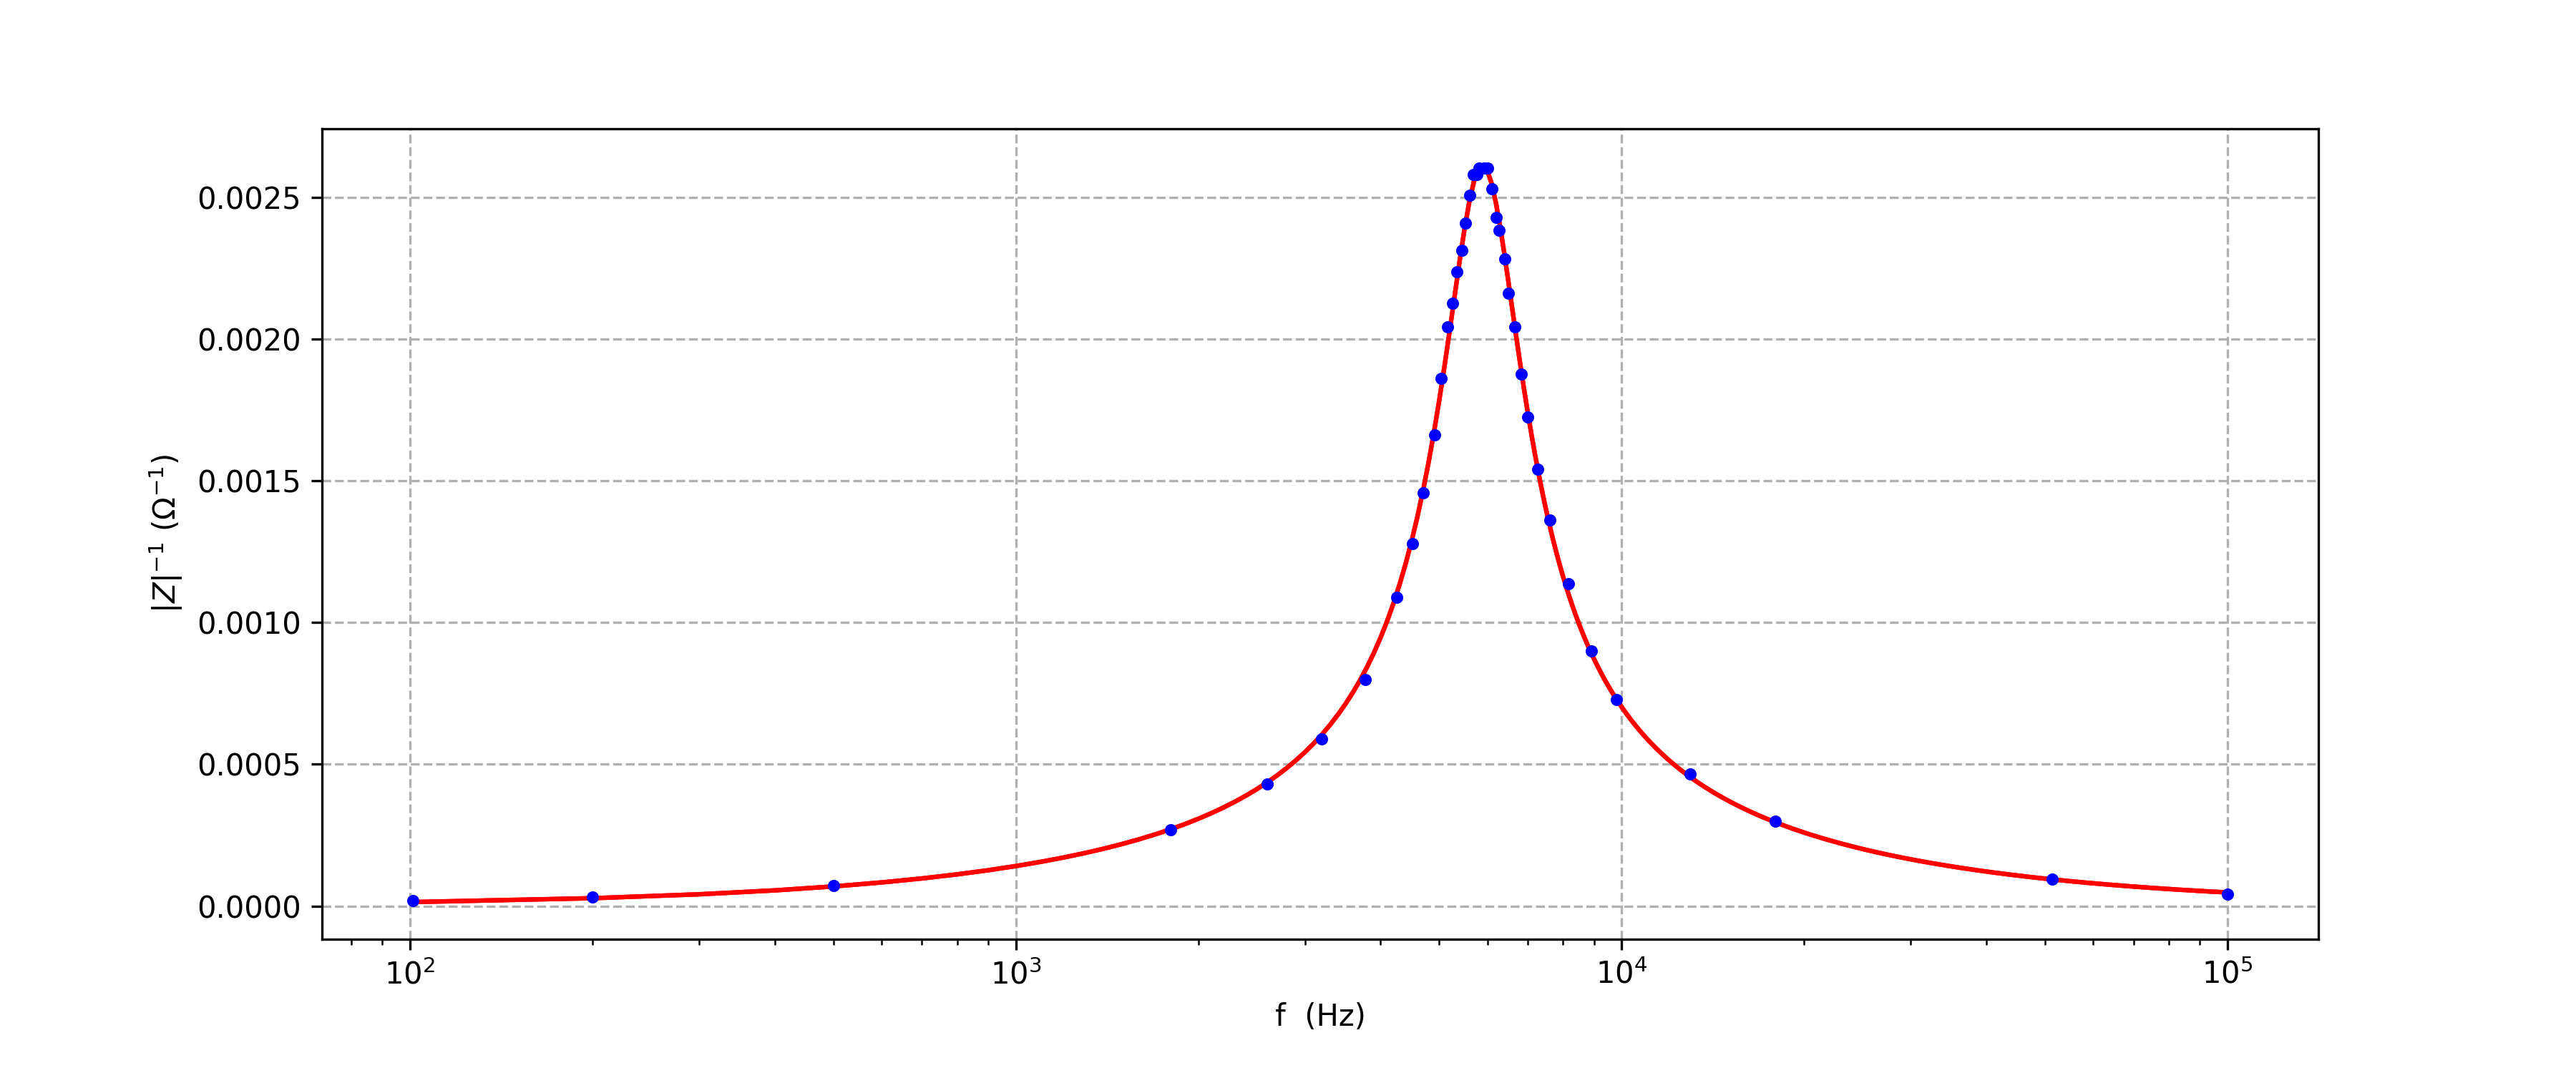
\includegraphics[scale=0.60]{plot5.png}
\caption{Representación de $|Z|^{-1}$ frente a $f$, sin barras de error y escala semi-logarítmica.}
\label{Fig:plot3}
\end{figure}

\subsubsection{Parte 2.2. Cálculo de $\tan (\phi)$}

Ahora trataremos de obtener $w_0$ y $Q$ usando los otros datos que nos faltán: los desfases. Sabemos por la ecuación \ref{Ec:z-y-arg(z)} que $\tan (\phi)$ se puede escribir como:

$$
\tan (\phi) =  - \dfrac{1}{R C w} + \dfrac{L}{R} w
$$

por lo que podemos hacer el ajuste:

\begin{equation}
\tan (\phi) = b_0 \dfrac{1}{w} + b_1 w \label{Ec:ajuste2}
\end{equation}

donde se puede ver que

\begin{equation}
b_0 = \dfrac{-1}{RC} \tquad b_1 = \dfrac{L}{R} \label{Ec:parametros2}
\end{equation}

y por lo tanto:

\begin{equation}
w_0= \sqrt{b_0/b_1} \tquad Q =  w_0 b_1 \label{Ec:valores2}
\end{equation}

Además tras hacer el ajuste veremos si dichos parámetros nos permiten deducir correctamente los valores de $\phi$, haciendo un ajuste de $f$ frente a $\phi$ y comparándolo con los resultados experimentales (figura \ref{Fig:plot5}). Una vez obtenido el ajuste \ref{Fig:plot4} podemos obtener\\

\begin{table}[h!] 	 \centering 
\begin{tabular}{|c|c|c|c|} 
\hline 
$b_0 \ (\Omega^{-1} F^{-1}) $  & $s(b_0) \ (\Omega^{-1} F^{-1})$ & $ b_1 \ (H/\Omega)$ & $s(b_1) \ (H/\Omega)$    \\ \hline 
$-12.4 \cdot 10^{4}$  & $-2.1 \cdot 10^{4}$ & $ 9.3 \cdot 10^{-5} $ & $1.3 \cdot 10^{-5} $ \\ 
\hline
\end{tabular} 
\caption{valores del ajuste \ref{Ec:ajuste2}} 
\label{Tab:regresion2} 
\end{table} 
 
 


Usando las ecuaciones \ref{Ec:valores2} podemos obtener directamente:\\
 
\begin{table}[h!] 	 \centering 
\begin{tabular}{|c|c|c|c|c|c|c|c|} 
\hline 
$Q \  $  & $s(Q) \ $ & $ B \ (k \Hz)$ & $s(B) \ (k \Hz)$ & $w_0 \ (\mathrm{rad}/s)  $ &  $s(w_0) \ (\mathrm{rad}/s)$  & $f_0 \ (k$Hz) & $s(f_0) \ (k$Hz) \\ \hline 
$3.39 $  & $0.60 $ & $ 1.72 $ & $0.36$ & $36.5 \cdot 10^3 $ & $4.0 \cdot 10^3 $ & 5.82 & 0.64 \\ 
\hline
\end{tabular} 
\caption{parámetros intrínsecos del circuito para el ajuste \ref{Ec:ajuste2}} 
\label{Tab:valores3} 
\end{table} 
 

Al igual que antes a la regresión \ref{Fig:plot4} le faltan algunos datos. Esto es por la misma razón que antes: los datos extremales presentan una elevada incertidumbre y solo complican hacer la regresión. En la figura \ref{Fig:plot5} presentamos todos los datos para que se pueda comprobar si los parámetros son capaces de ajustar aquellos valores que no fueron incluidos:


\begin{figure}[h!] \centering
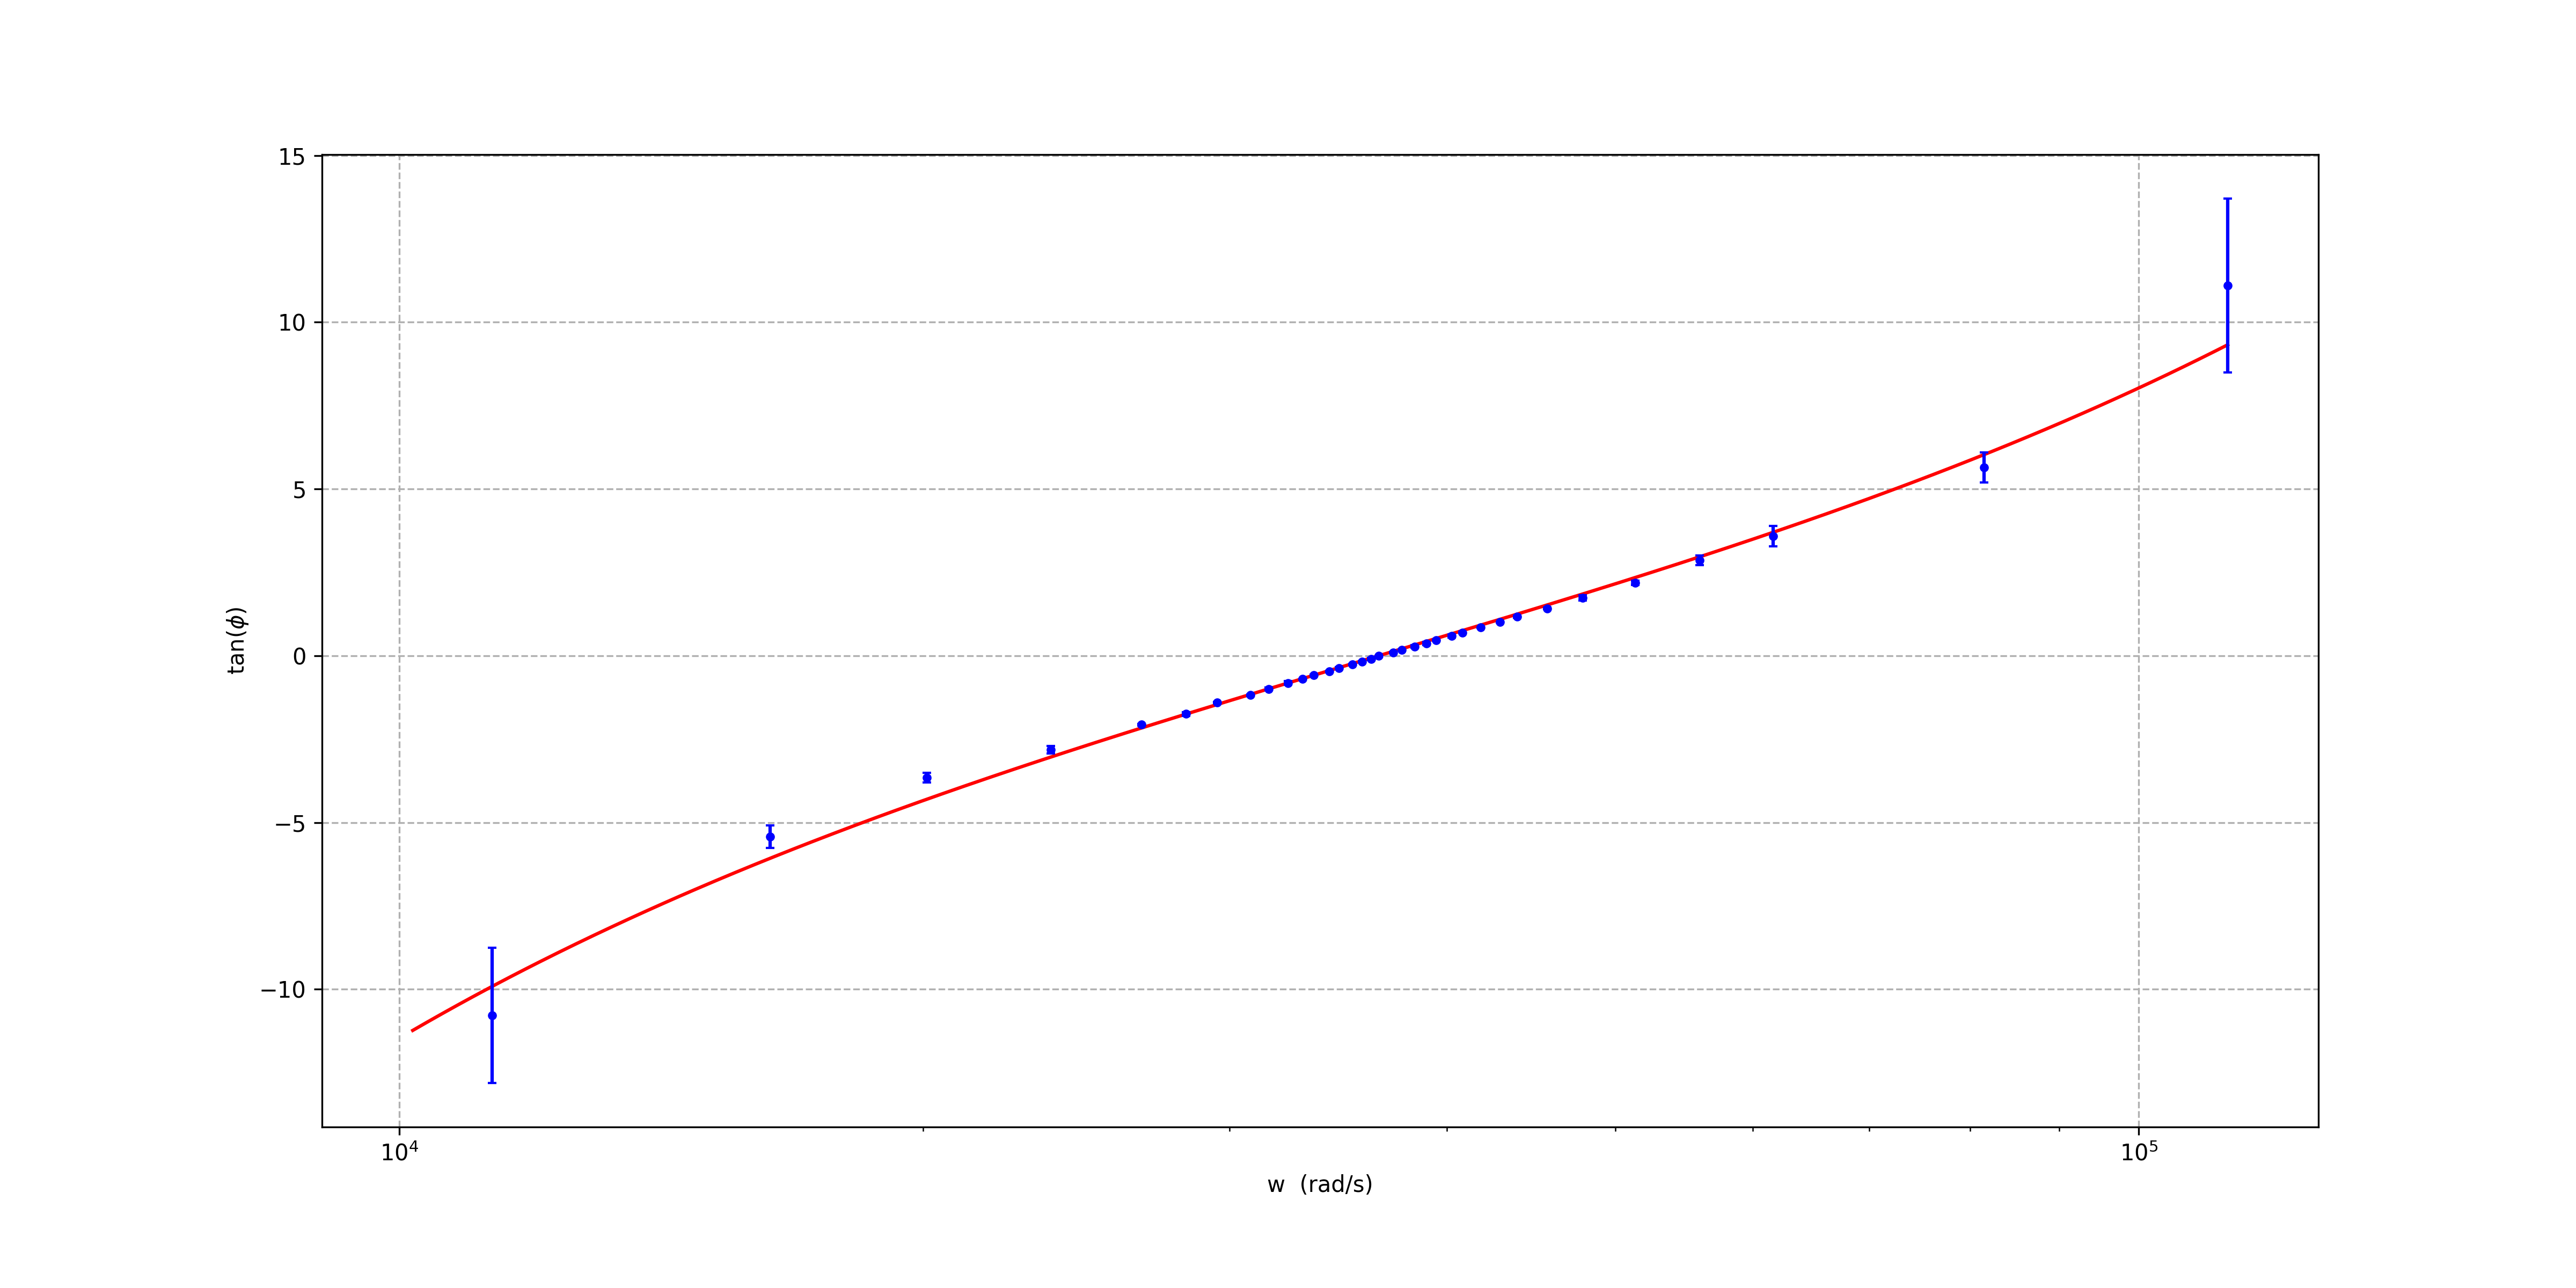
\includegraphics[scale=0.45]{plot3.png}
\caption{representación y ajuste de $\tan(\phi)$ frente a $w$}
\label{Fig:plot4}
\end{figure}



\begin{figure}[h!] \centering
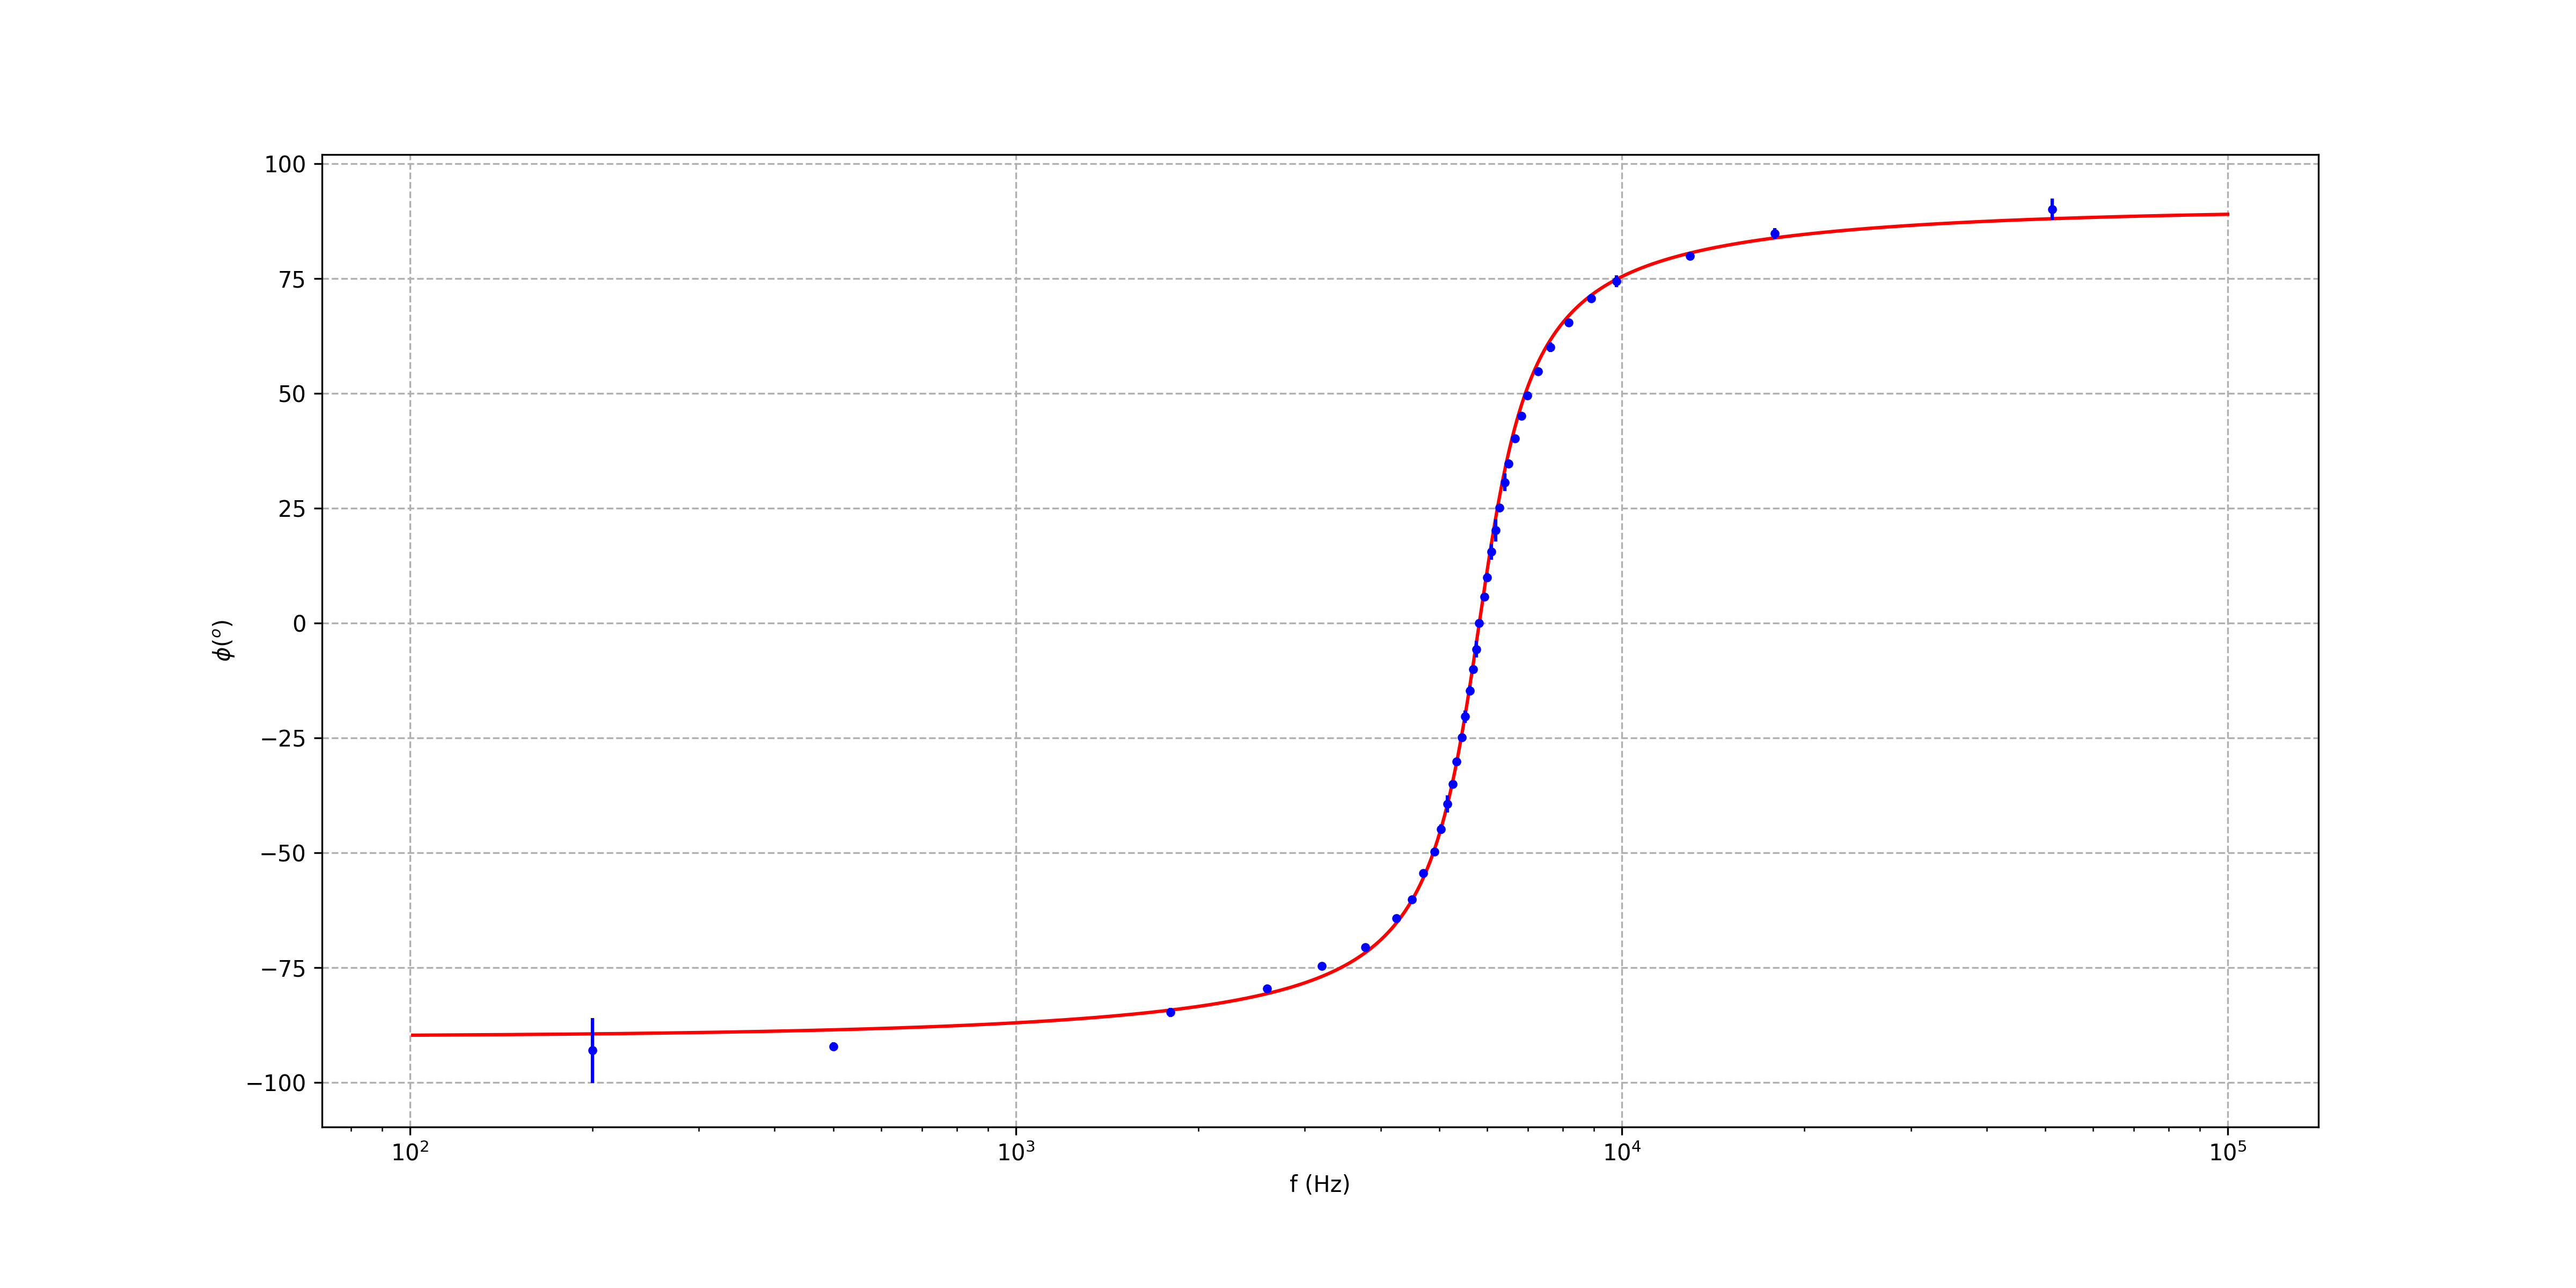
\includegraphics[scale=0.45]{plot4.png}
\caption{representación y ajuste de $\phi$ frente a $f$}
\label{Fig:plot5}
\end{figure}

\subsection{Parte 3. Análisis teórico.}

Ahora vamos a analizar un momento los resultados obtenidos directamente de las medidas del laboratorio $w_0$, $B$ y $Q$. Entonces como ya mencionamos tenemos que $w_0$ es la frecuencia para la cual el desfase es nulo:

\begin{equation}
w_0 = 36568 \mathrm{rad}/s \tquad s(w_0) = 63 \ \mathrm{rad}/s
\end{equation}
El valor de $B$ es aquel valor para el cual la amplitud de la señal de entrada decae en relación a $1/\sqrt{2}$ , o cuando el desfase es igual a $45 ^o$. Como no tenemos los datos fijos de 45 y -45 Hacemos interpolación lineal entre los valores que se encuentran. De aquí podemos obtener finalmente que el ancho de banda experimental es:

\begin{equation}
B =  1791 \Hz \tquad sB = 41 \Hz
\end{equation}

Por lo tanto podemos obtener que:

\begin{equation}
Q = 3.249 \tquad s(Q) =  0.082
\end{equation}

Estos son los valores teóricos que podemos medir.

\section{Conclusiones}

En este apartado analizaremos si hemos cumplido el objetivo de esta práctica. \\

Primero analicemos los datos empíricos, comparando los parámetros teóricos con los parámetros obtenidos haciendo las regresion, para luego estudiar los obtenidos experimentalmente.\\

Comparamos la resistencia, la capacidad y la auto-inductancia en la tabla \ref{Tab:conclusion1}; y el factor de calidad, frecuencia de corte y ancho de banda en la tabla \ref{Tab:conclusion2}:

\begin{table}[h!] 	 \centering 
\begin{tabular}{c|c|c|c|c|c|c|} 

  & \cellcolor{color1} $ R \  (\Omega) $  &  \cellcolor{color1}  $s(R) \ (\Omega) $  &  \cellcolor{color1} $ C \ (nF)  $ & \cellcolor{color1}  $s(C) \ (nF)$  & \cellcolor{color1} $L \ (mH)$ & \cellcolor{color1} $s(L) \ (mH)$ \\ \hline 
 \cellcolor{color1} Parte 1 & \cellcolor{color2} $ 345.8 $  &  \cellcolor{color2} $3.6 $  &  \cellcolor{color2} $22.00  $ &  \cellcolor{color2} $ 1.10 $ &   \cellcolor{color2}33.00 &  \cellcolor{color2} 1.65  \\ \hline  
 \cellcolor{color1} Parte 2.1 &  \cellcolor{color2} $ 383 $  &  \cellcolor{color2} $88 $  &  \cellcolor{color2} $ 21.88  $ &  \cellcolor{color2} $ 0.36 $ &  \cellcolor{color2}  33.35 &  \cellcolor{color2} 0.48  \\ \hline  
 \cellcolor{color1} Parte 2.2 2&  \cellcolor{color2} - & \cellcolor{color2} - & \cellcolor{color2} - &  \cellcolor{color2} - & \cellcolor{color2} - & \cellcolor{color2} - \\ \hline  
 \cellcolor{color1} Experimentales &  \cellcolor{color2} - & \cellcolor{color2} - & \cellcolor{color2} - &  \cellcolor{color2} - & \cellcolor{color2} - & \cellcolor{color2} - \\ 
\hline
\end{tabular} 
\caption{comparación de los parámetros intrínsecos del circuito} 
\label{Tab:conclusion1} 
\end{table} 

\begin{table}[h!] 	 \centering 
\begin{tabular}{c|c|c|c|c|c|c|} 

  & \cellcolor{color3} $ Q \   $  & \cellcolor{color3}   $s(Q)  $  & \cellcolor{color3}  $ B \ (\Hz)  $ & \cellcolor{color3}  $s(B) \ (\Hz)$  & \cellcolor{color3} $ w_0 \ (\mathrm{rad}/s)$ &  \cellcolor{color3} $s(w_0) \ (\mathrm{rad}/s)$ \\ \hline 
  \cellcolor{color3} Parte 1 &  \cellcolor{color4} $ 3.54 $  & \cellcolor{color4} $0.22 $  & \cellcolor{color4} $1667  $  & \cellcolor{color4} $ 119 $ &  \cellcolor{color4} 37100 & \cellcolor{color4} 1300  \\ \hline 
 \cellcolor{color3} Parte 2.1 & \cellcolor{color4} $ 3.22 $  & \cellcolor{color4} $0.75 $  & \cellcolor{color4} $1828  $ & \cellcolor{color4}$ 427 $ & \cellcolor{color4} 37020 &  \cellcolor{color4} 810  \\ \hline 
 \cellcolor{color3} Parte 2.2 & \cellcolor{color4} $ 3.39 $  & \cellcolor{color4} $0.60 $  & \cellcolor{color4} $1717  $ & \cellcolor{color4}$ 359 $ & \cellcolor{color4} 36500 &\cellcolor{color4} 4000  \\ \hline  
 \cellcolor{color3} Experimentales & \cellcolor{color4} $ 3.249 $  & \cellcolor{color4} $0.083 $  & \cellcolor{color4} $ 1791  $ & \cellcolor{color4} $ 41 $ & \cellcolor{color4} 36568 & \cellcolor{color4} 63  \\  
\hline
\end{tabular} 
\caption{comparación de los parámetros intrínsecos del circuito} 
\label{Tab:conclusion2} 
\end{table} 
 
Menciono que las cifras significativas están mal en los t res primeros valores de la frecuencia de corte y en el valor del ancho de banda para la parte 2.2. Esto responde únicamente a fines estéticos, solo queremos comparar los datos. En las otras tablas se realizo de manera correcta. \\

 
Como podemos ver en la tabla \ref{Tab:conclusion1} los datos obtenidos mediante las regresiones son sumamente parecidos entre sí, sobretodo las capacidades y las autoinductancias, estando entre sus rangos de incertidumbre. La resistencia sin embargo difiere un poco, lo cual es normal, ya que en el calculo de la parte 1 solo hemos tenido en cuenta las resistencias del bobinado y la resistencia, sin ver nada respecto los cables, el resto del circuito y el propio osciloscopio, por lo que es normal que aumente un poco. De todos modos se parecen bastante, coincidiendo en el orden, con una diferencia relativa de solo un 10\%. Aunque es demasiado pronto para sacar las conclusiones (aun nos queda analizar los otros resultados) podemos empezar a decir que realmente la teoría de circuitos si es una buena aproximación. \\

En la tabla \ref{Tab:conclusion2} ocurre exactamente lo mismo. En este caso tenemos mas valores, que hemos calculado de manera diferente, pero tenemos algo mucho mas significativo: los datos experimentales medidos directamente. Y lo que obtenemos es que los parámetros son muy similares, por lo que realmente si podemos obtener información usando dicha teoría. \\

Por otra parte sería muy complicado mejorar esta práctica, y de hecho incluir otras fuentes de incertidumbre como las dadas por la inductancia del propio osciloscopio, las dadas por la calibración... sería un proceso largo y tedioso, que sale fuera de lo que se pretende en esta práctica: tener mas fuentes de incertidumbre no nos llevará a rechazar o no la teoría de circuitos, ya que sabemos que esta es solo una aproximación. La verdaderas fuentes de incertidumbre están en la propia forma de entender el problema. Sin embargo esto no nos importa: sabemos que va a existir un error. Lo que nos importa es que si sirve como una primera aproximación. \\

Además queda demostrado que un circuito RLC actúa como un filtro de señal, ya que toda señal con frecuencia no cercana a la frecuencia de resonancia se destruirá por interferencia destructiva de los desfases del condensador y la bobina. 




\section{Bibliografía} \label{Sec:7}

\begin{enumerate}
\item \textbf{Victor Pardo}. \textit{Apuntes electro II 2016, tema 7.}
\item \textbf{Paco Ares}. \textit{Apuntes electro II, 2023, tema 4.}
\item \textit{Guion de prácticas Tecnicas II, 2023, Práctica 1.}
\end{enumerate}

Además cabe mencionar a los guiones de Andres Novo, Andrea Ferrer y Sara González para resolver alguna duda puntual. Consultar la página de scipy optimize. \footnote{\textcolor{blue}{\url{https://docs.scipy.org/doc/scipy/reference/optimize.html}}}.

\newpage 


\section{Datos}


\begin{table}[h!] 	 \centering 
\begin{tabular}{|c|c|c|c|c|c|c|c|} 

\hline 
$f  \ (\Hz) $  & $s(f) \ (\Hz)$ & $ w \ (\mathrm{rad}/s)$ & $s(w) \ (\mathrm{rad}/s)$ & $V_1 \ (V)  $ &  $s(V_1) \ (V)$ & $V_2 \ (V)$ & $ s(V_2) \ (V)$ \\ \hline 
100000  & 10 &  628318 & 63 & 0.1588 & 0.0099 & 10.80 & 0.64 \\ 
51350  & 10 &  322641 & 63 & 0.334 & 0.019 & 10.16 & 0.61 \\ 
17900  & 10 &  112469 & 63 & 1.040 & 0.054 & 10.08 & 0.60 \\ 
12970  & 10 &  81492 & 63 & 1.620 & 0.083 & 10.08 & 0.60 \\ 
9810  & 10 &  61638 & 63 & 2.50 & 0.13 & 9.92 & 0.60 \\ 
8900  & 10 &  55920 & 63 & 3.06 & 0.16 & 9.84 & 0.59 \\ 
8170  & 10 &  51333 & 63 & 3.84 & 0.19 & 9.76 & 0.59 \\ 
7620  & 10 &  47877 & 63 & 4.56 & 0.23 & 9.68 & 0.58 \\ 
7270  & 10 &  45678 & 63 & 5.12 & 0.26 & 9.60 & 0.58 \\ 
6990  & 10 &  43919 & 63 & 5.68 & 0.29 & 9.52 & 0.58 \\ 
6830  & 10 &  42914 & 63 & 6.08 & 0.31 & 9.36 & 0.57 \\ 
6660  & 10 &  41846 & 63 & 6.56 & 0.33 & 9.28 & 0.56 \\ 
6500  & 10 &  40840 & 63 & 6.88 & 0.35 & 9.20 & 0.56 \\ 
6410  & 10 &  40275 & 63 & 7.20 & 0.36 & 9.12 & 0.56 \\ 
6280  & 10 &  39458 & 63 & 7.52 & 0.38 & 9.12 & 0.56 \\ 
6200  & 10 &  38955 & 63 & 7.60 & 0.38 & 9.04 & 0.55 \\ 
6100  & 10 &  38327 & 63 & 7.84 & 0.39 & 8.96 & 0.55 \\ 
6000  & 10 &  37699 & 63 & 8.00 & 0.40 & 8.88 & 0.54 \\ 
5930  & 10 &  37259 & 63 & 8.00 & 0.40 & 8.88 & 0.54 \\ 
5820  & 10 &  36568 & 63 & 8.00 & 0.40 & 8.88 & 0.54 \\ 
5760  & 10 &  36191 & 63 & 8.00 & 0.40 & 8.96 & 0.55 \\ 
5690  & 10 &  35751 & 63 & 8.00 & 0.40 & 8.96 & 0.55 \\ 
5620  & 10 &  35311 & 63 & 7.84 & 0.39 & 9.04 & 0.55 \\ 
5520  & 10 &  34683 & 63 & 7.60 & 0.38 & 9.12 & 0.56 \\ 
5450  & 10 &  34243 & 63 & 7.36 & 0.37 & 9.20 & 0.56 \\ 
5340  & 10 &  33552 & 63 & 7.12 & 0.36 & 9.20 & 0.56 \\ 
5260  & 10 &  33049 & 63 & 6.80 & 0.34 & 9.24 & 0.56 \\ 
5160  & 10 &  32421 & 63 & 6.56 & 0.33 & 9.28 & 0.56 \\ 
5030  & 10 &  31604 & 63 & 6.08 & 0.31 & 9.44 & 0.57 \\ 
4910  & 10 &  30850 & 63 & 5.52 & 0.28 & 9.60 & 0.58 \\ 
4700  & 10 &  29530 & 63 & 4.88 & 0.25 & 9.68 & 0.58 \\ 
4510  & 10 &  28337 & 63 & 4.32 & 0.22 & 9.76 & 0.59 \\ 
4250  & 10 &  26703 & 63 & 3.68 & 0.19 & 9.76 & 0.59 \\ 
3770  & 10 &  23687 & 63 & 2.74 & 0.14 & 9.92 & 0.60 \\ 
3200  & 10 &  20106 & 63 & 2.04 & 0.10 & 10.00 & 0.60 \\ 
2600  & 10 &  16336 & 63 & 1.500 & 0.077 & 10.06 & 0.60 \\ 
1800  & 10 &  11309 & 63 & 0.936 & 0.049 & 10.08 & 0.60 \\ 
500  & 10 &  3144 & 63 & 0.248 & 0.014 & 10.08 & 0.60 \\ 
200  & 10 &  1256 & 63 & 0.1090 & 0.0074 & 10.16 & 0.61 \\ 
101  & 10 &  635 & 63 & 0.0645 & 0.0052 & 10.48 & 0.62 \\ 
\hline
\end{tabular} 
\caption{datos de la practica} 
\label{Tab:datos1} 
\end{table} 
 
\begin{table}[h!] 	 \centering 
\begin{tabular}{|c|c|c|c|c|c|} 
\hline 
$f  \ (\Hz) $  & $s(f) \ (\Hz)$ & $ \phi \ (^o)$ & $s(\phi) \ (^o)$ & $Z \ (k \Omega)  $ &  $s(Z) \ (k \Omega)$ \\ \hline 
100000  & 10 &  89.00 & 4.24 & 23.5 & 2.0 \\ 
51350  & 10 &  90.06 & 2.34 & 10.52 & 0.87 \\ 
17900  & 10 &  84.85 & 1.20 & 3.35 & 0.27 \\ 
12970  & 10 &  79.95 & 0.78 & 2.15 & 0.17 \\ 
9810  & 10 &  74.40 & 1.27 & 1.37 & 0.11 \\ 
8900  & 10 &  70.71 & 0.89 & 1.112 & 0.088 \\ 
8170  & 10 &  65.45 & 0.64 & 0.879 & 0.070 \\ 
7620  & 10 &  60.05 & 1.06 & 0.734 & 0.058 \\ 
7270  & 10 &  54.87 & 0.38 & 0.648 & 0.051 \\ 
6990  & 10 &  49.60 & 0.71 & 0.580 & 0.046 \\ 
6830  & 10 &  45.11 & 0.42 & 0.532 & 0.042 \\ 
6660  & 10 &  40.16 & 0.36 & 0.489 & 0.039 \\ 
6500  & 10 &  34.76 & 0.91 & 0.462 & 0.037 \\ 
6410  & 10 &  30.65 & 1.91 & 0.438 & 0.035 \\ 
6280  & 10 &  25.10 & 0.71 & 0.419 & 0.033 \\ 
6200  & 10 &  20.25 & 2.47 & 0.411 & 0.033 \\ 
6100  & 10 &  15.55 & 1.77 & 0.395 & 0.032 \\ 
6000  & 10 &  10.00 & 0.99 & 0.384 & 0.031 \\ 
5930  & 10 &  5.75 & 0.64 & 0.384 & 0.031 \\ 
5820  & 10 &  0.00 & 0.01 & 0.384 & 0.031 \\ 
5760  & 10 &  -5.65 & 1.77 & 0.387 & 0.031 \\ 
5690  & 10 &  -10.00 & 0.71 & 0.387 & 0.031 \\ 
5620  & 10 &  -14.65 & 1.06 & 0.399 & 0.032 \\ 
5520  & 10 &  -20.35 & 1.34 & 0.415 & 0.033 \\ 
5450  & 10 &  -24.90 & 0.71 & 0.432 & 0.034 \\ 
5340  & 10 &  -30.15 & 0.78 & 0.447 & 0.036 \\ 
5260  & 10 &  -35.05 & 0.07 & 0.470 & 0.037 \\ 
5160  & 10 &  -39.35 & 1.91 & 0.489 & 0.039 \\ 
5030  & 10 &  -44.85 & 1.06 & 0.537 & 0.043 \\ 
4910  & 10 &  -49.80 & 0.71 & 0.601 & 0.048 \\ 
4700  & 10 &  -54.40 & 0.28 & 0.686 & 0.054 \\ 
4510  & 10 &  -60.20 & 0.85 & 0.781 & 0.062 \\ 
4250  & 10 &  -64.20 & 0.28 & 0.917 & 0.073 \\ 
3770  & 10 &  -70.50 & 0.71 & 1.252 & 0.099 \\ 
3770  & 10 &  -70.50 & 0.71 & 1.25 & 0.10 \\ 
3200  & 10 &  -74.70 & 0.57 & 1.70 & 0.13 \\ 
2600  & 10 &  -79.55 & 0.64 & 2.32 & 0.18 \\ 
1800  & 10 &  -84.70 & 0.99 & 3.72 & 0.30 \\ 
500  & 10 &  -92.15 & 0.92 & 14.1 & 1.2 \\ 
200  & 10 &  -93.00 & 7.07 & 32.2 & 2.9 \\ 
101  & 10 &  -100.00 & 4.24 & 56.2 & 5.7 \\ 
\hline
\end{tabular} 
\caption{datos de la práctica} 
\label{Tab:datos2} 
\end{table} 
 
 
 
 
\end{document}
